

\chapter{Процедуры и схемы сбора установок и стендов}
\label{cha:appendix_schemes}


Схема стенда для проверки выполнения требований назначения приведена на рис.~\ref{fig:xkcd}. 

\section{Раздел в приложении}

Перечень оборудования, задействованного в стенде на рис. \ref{fig:xkcd} приведен в табл.~\ref{tab:stend_eqip}.
	
	\begin{figure}[H]
		\centering
		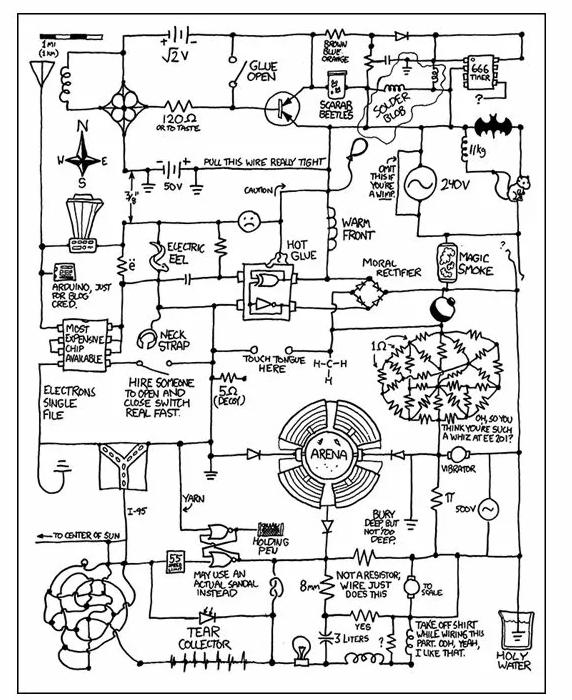
\includegraphics[width=0.75\textwidth]{inc/img/appx/xkcd}
		\caption{Схема стенда прямиком с xkcd! Заодно это пример растрового рисунка}
		\label{fig:xkcd}
	\end{figure}
	
\textit{Примечание. Какое-нибудь примечание.}
	
	\begin{longtable}{|c|p{4cm}|p{11cm}|}
		\caption{Перечень оборудования, задействованного в стенде на рис. \ref{fig:xkcd}} \label{tab:stend_eqip}\\
		\hline 
		№ & Обозначение & Тип и характеристики  \\		
		\endfirsthead
		\multicolumn{3}{r}{... продолжение таблицы \ref{tab:stend_eqip}}\\ [1em] % отступ до таблицы
		\hline 
		№ & Обозначение & Тип и характеристики  \\
		\endhead
		\hline
		
		1 &  ПРМ                       & Приемник навигационных сигналов ГНСС заданных типов \\ 
		\hline 
		
		2 &  ИС  &  Имитатор навигационных сигналов, R\&S SMBV100B c не менее чем 32 каналами имитации (опции SMBVB-K136, SMBVB-K137), опциями формирования сигналов ГНСС SMBVB-K44, SMBVB-K62, SMBVB-K66, SMBVB-K94, SMBVB-K98, SMBVB-K107, опциями частотных диапазонов SMBVB-K134, SMBVB-K135.
		\\ 
		\hline 
		
		3 & Д                         & Радиочастотный сумматор-делитель мощности MiniCircuits ZAPD-2DC-S+  \\
		\hline
		
		4 & АС                         & Анализатор спектра R\&S FSV \\
		\hline
		
		5 & ИП                         & Лабораторный источник питания R\&S HAMEG HMP4040 \\
		\hline
		
		6 & ПК                         & Персональный компьютер: 
		\begin{itemize}
			\item процессор семейства Intel Core i3 и выше; 
			\item от 8 Гб оперативной памяти;
			\item наличие интерфейса Ethernet;
			\item ОС Linux Kubuntu версии от 16.04;
			\item ПО Matlab, python версии 3 и выше.
		\end{itemize} 
		\\ 
		\hline 
		
		7 & КОМ & Коммутатор (switch) Ethernet 100 Мбит/с, минимум 4 порта \\ 
		\hline 
		
		8 & -          & Кабельные сборки из состава Комплекта кабелей испытуемого образца (отмечены синим)  \\ 
		\hline 
		
		9 & -          & Дополнительные кабельные сборки и адаптеры: радиочастотных, питания, цифровых интерфейсов (отмечены красным, адаптеры могут применяться к синим) \\ 
		\hline 

		10 & -         & Табличка может быть очень длинной, с переносом на следующую страницу \\ 
		\hline 		
		
	\end{longtable}

%%% Local Variables: 
%%% mode: latex
%%% TeX-master: "rpz"
%%% End: 
